\documentclass[a4paper]{article}
\usepackage{amsmath}
\usepackage{amssymb}
\usepackage{braket}%量子力学符号
\usepackage{geometry}
\usepackage{enumerate}
\usepackage{natbib}
\usepackage{float}%稳定图片位置
\usepackage{graphicx,subfig}%画图
\usepackage{caption}
\usepackage[english]{babel}
\usepackage{indentfirst}%缩进
\usepackage{enumerate}%加序号
\usepackage{multirow}%合并行
\usepackage{hyperref}
\hypersetup{hypertex=true, colorlinks=true, linkcolor=black, anchorcolor=black, citecolor=black}
\title{\Large \textbf{VP390 Problem Set 4}\\
\author{\textbf{Pan, Chongdan ID:516370910121}\\
}
}
\begin{document}
\maketitle
\section{Problem 1}
\begin{enumerate}[(a)]
    \item $\hat{\pi_x}f(x)=\hbar\frac{\partial e^{-x^2}}{\partial x}=-2x\hbar e^{-x^2}$
    \\$\hat{M}_{\frac{1}{2}}f=e^{-(\frac{1}{2}x)^2}=e^{-\frac{x^2}{4}}$
    \item Assume the conjugates exist and donate as $\hat{\pi_x}^\dagger,\hat{M_c}^\dagger$
    \\$\braket{\Psi,\hat{\pi_x}\Phi}=\int_{-\infty}^\infty\Psi^*\hbar\frac{\partial\Phi}{\partial x}\mathrm{d}x$
    \\$=[\hbar\Psi^*\Phi]^\infty_{-\infty}-\int_{-\infty}^\infty\hbar\frac{\partial\Psi^*}{\partial x}\Phi\mathrm{d}x=-\braket{\hat{\pi_x}\Psi,\Phi}$
    \\So $\hat{\pi_x}^\dagger=-\hat{\pi_x}$, and it's not Hermitian
    \\\\$\braket{\Psi,\hat{M_c}\Phi}=\int_{-\infty}^\infty\Psi^*(x)\Phi(cx)\mathrm{d}x$
    \\Let $y=cx$, then $\braket{\Psi,\hat{M_c}\Phi}=\int_{-\infty}^\infty\frac{\Psi^*(\frac{y}{c})\Phi(y)}{c}\mathrm{d}y$
    \\So $\hat{M_c}^\dagger=\frac{\hat{M_{1/c}}}{c}$, and it's not Hermitian
\end{enumerate}
\section{Problem 2}
\begin{enumerate}[(a)]
    \item $\braket{\Psi,(\alpha\hat{A})\Phi}=\alpha\braket{\hat{A}^\dagger\Psi,\Phi}=\braket{(\alpha^*\hat{A}^\dagger)\Psi,\Phi}$
    \\So $(\alpha\hat{A})^\dagger=\alpha^*\hat{A}^\dagger$
    \item $\braket{\Psi,\hat{A}\Phi}=\braket{\hat{A}^\dagger\Psi,\Phi}=\braket{\Phi,\hat{A}^\dagger\Psi}=\braket{(\hat{A}^\dagger)^\dagger\Phi,\Psi}=\braket{\Psi,(\hat{A}^\dagger)^\dagger\Phi}$
    \\So $(\hat{A}^\dagger)^\dagger=\hat{A}$
    \item $\braket{(\hat{A}\hat{B})^\dagger\Psi,\Phi}=\braket{\Psi,(\hat{A}\hat{B})\Phi}=\braket{\Psi,\hat{A}(\hat{B}\Phi)}=\braket{\hat{A}^\dagger\Psi,\hat{B}\Phi}=\braket{\hat{B}^\dagger\hat{A}^\dagger\Psi,\Phi}$
    \\So $(\hat{A}\hat{B})^\dagger=\hat{B}^\dagger\hat{A}^\dagger$
\end{enumerate}
\section{Problem 3}
\begin{enumerate}[(a)]
    \item $E_1=\frac{\hbar^2\pi^2}{2mL^2}=\frac{(1.05\times10^{-34})^2\times3.14^2}{2\times1.67\times10^{-27}(10^{-15})^2}\approx3.25\times10^{-11}J=203.4$MeV
    \item $E_1=h\nu=h\frac{c}{\lambda}$
    \\$\lambda_1=h\frac{c}{E_1}=6.63\times10^{-34}\frac{3\times10^8}{3.3\times10^{-11}}\approx6.12\times10^{-15}$m
    \item $\bigtriangleup E=(2^2-1)E_1=3E_1$
    \\$\lambda_2=\frac{\lambda_1}{3}\approx2.04\times10^{-15}$m
    \item $\bigtriangleup E=(3^2-2^2)E_1=5E_1$
    \\$\lambda_3=\frac{\lambda_1}{5}\approx1.22\times10^{-15}$m
    \item $\bigtriangleup E=(3^2-1)E_1=8E_1$
    \\$\lambda_4=\frac{\lambda_1}{8}\approx7.65\times10^{-16}$m
\end{enumerate}
\section{Problem 4}
\begin{enumerate}[(a)]
    \item $\braket{\Psi,\Psi}=\braket{\sqrt{\frac{1}{3}}\psi_3,\sqrt{\frac{1}{3}}\psi_3}+\braket{\sqrt{\frac{1}{3}}\psi_3,\sqrt{\frac{2}{3}}\psi_5}+\braket{\sqrt{\frac{2}{3}}\psi_5,\sqrt{\frac{1}{3}}\psi_3},\braket{\sqrt{\frac{2}{3}}\psi_5+\sqrt{\frac{2}{3}}\psi_5}$
    \\$=\frac{1}{3}\braket{\psi_3,\psi_3}+0+0+\frac{2}{3}\braket{\psi_5,\psi_5}=\frac{1}{3}+\frac{2}{3}=1$
    \\So it's normalized
    \item $\Psi(x,0)=\sqrt{\frac{2}{3a}}\sin\frac{3\pi}{a}x+\sqrt{\frac{4}{3a}}\sin\frac{5\pi}{a}x$
    \\$\Psi(x,0)\Psi(x,0)^*=(\sqrt{\frac{2}{3a}}\sin\frac{3\pi}{a}x+\sqrt{\frac{4}{3a}}\sin\frac{5\pi}{a}x)^2$
    \\$=\frac{2}{3a}\sin^2\frac{3\pi}{a}x+\frac{2\sqrt{2}}{3a}\sin\frac{3\pi}{a}x\sin\frac{5\pi}{a}x+\frac{4}{3a}\sin^2\frac{5\pi}{a}x$
    \\$\int_0^{a/2}\Psi(x,0)^2\mathrm{d}x=\frac{4}{15}$
    \\So the probability is $\frac{1}{2}$
    \item The possible outcome of energy is $E_3=\frac{9\hbar^2\pi^2}{2ma^2},E_5=\frac{25\hbar^2\pi^2}{2ma^2}$
    \\The probability to get $E_3$ is $\frac{1}{3}$, for $E_5$ is $\frac{2}{3}$
    \item $E=\frac{1}{3}E_3+\frac{2}{3}E_5=\frac{59\hbar^2\pi^2}{6ma^2}$
    \item $\Psi(x,t)=\sqrt{\frac{1}{3}}e^{\frac{i}{\hbar}E_3t}\psi_3(x)+\sqrt{\frac{2}{3}}e^{\frac{i}{\hbar}E_5t}\psi_5(x)$
\end{enumerate}
\section{Problem 5}
\begin{enumerate}[(a)]
    \item $\Psi(x,0)=\Phi(x)=\sum_nc_n\psi_n(x)$, where 
    \\$\Phi(x)=\begin{cases}
        \sqrt{\frac{2}{a}}\sin\frac{\pi}{a}x &0\leq x\leq a\\
        0 &\mathrm{otherwise}
    \end{cases}$
    \\$c_m=\braket{\psi_m,\Phi}$, where
    \\$\psi_m(x)=\begin{cases}
        \sqrt{\frac{2}{2a}}\sin\frac{m\pi}{2a}x &0\leq x\leq 2a\\
        0 &\mathrm{otherwise}
    \end{cases}$
    \\$c_m=\int_{-\infty}^{\infty}\psi_m^*\Phi\mathrm{d}x=\frac{\sqrt{2}}{a}\int_0^a\sin\frac{\pi}{a}x\sin\frac{m\pi}{2a}x\mathrm{d}x$
    \\Therefore $c_1=\frac{4\sqrt{2}}{3\pi},c_2=\frac{\sqrt{2}}{2},c_3=\frac{4\sqrt{2}}{5\pi},c_4=0,c_5=\frac{-4\sqrt{2}}{21\pi}$
    \\When $0=t_1<t_2<t_3<t_4$, we can the plot:
    \begin{figure}[H]
        \centering
        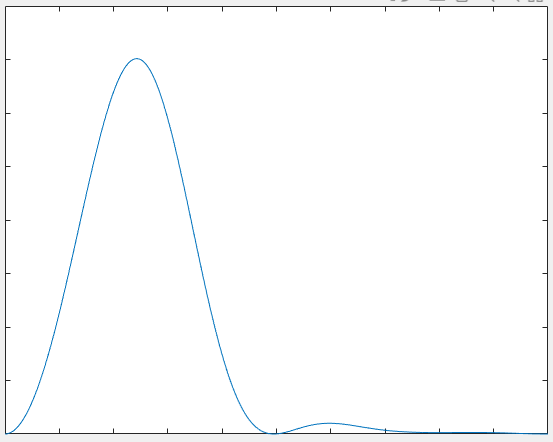
\includegraphics[scale=0.5]{P1.png}
        \caption{Plot for $t=t_1=0$}
        \label{P1}
    \end{figure}
    \begin{figure}[H]
        \centering
        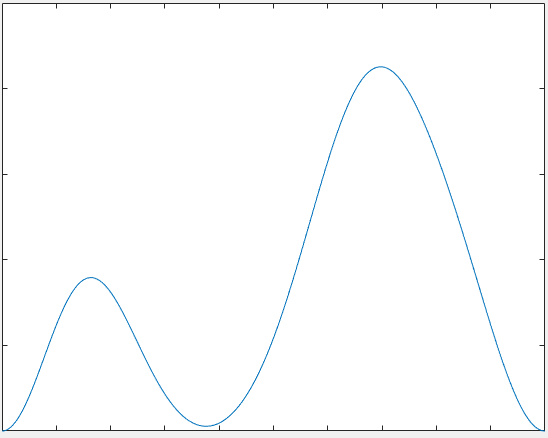
\includegraphics[scale=0.5]{P2.png}
        \caption{Plot for $t=t_2$}
        \label{P2}
    \end{figure}
    \begin{figure}[H]
        \centering
        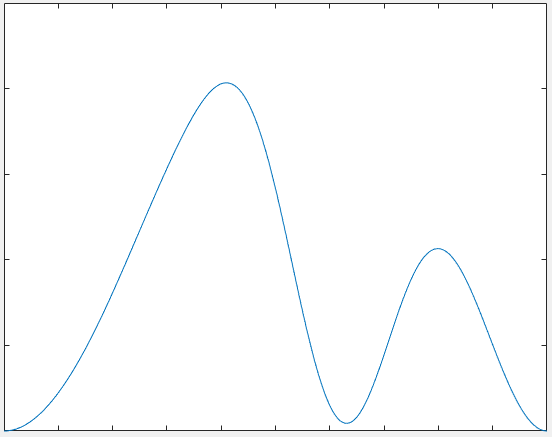
\includegraphics[scale=0.5]{P3.png}
        \caption{Plot for $t=t_3$}
        \label{P3}
    \end{figure}
    \begin{figure}[H]
        \centering
        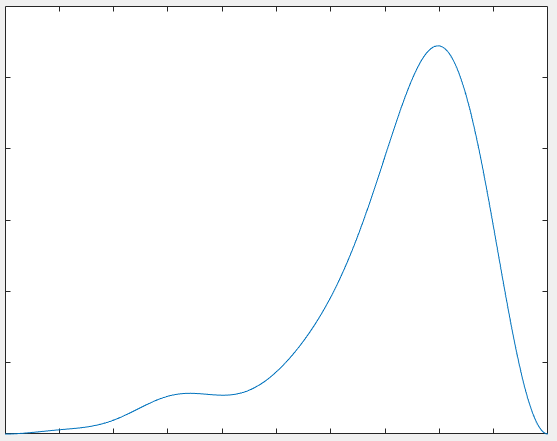
\includegraphics[scale=0.5]{P4.png}
        \caption{Plot for $t=t_4$}
        \label{P4}
    \end{figure}
    \item When $t<0,E=\frac{\hbar^2\pi^2}{2ma^2}$
    \\When $t\geq0,E_2=\frac{\hbar^2\pi^2}{2m(2a)^2}n^2=E$
    \\So the probability is $c_2^2=0.5$
\end{enumerate}
\section{Problem 6}
\begin{enumerate}[(b)]
    \item Assume $\psi$ is the solution for $-\frac{\hbar^2}{2m}\frac{\mathrm{d}^2\psi(x)}{\mathrm{d}x^2}+V(x)\psi(x)=E\psi(x)$
    \\Then $-\frac{\hbar^2}{2m}\frac{\mathrm{d}^2\psi(-x)}{\mathrm{d}x^2}+V(-x)\psi(-x)=E\psi(-x)$
    \\Since $V(x)=V(-x)$
    \\$-\frac{\hbar^2}{2m}\frac{\mathrm{d}^2\psi(-x)}{\mathrm{d}x^2}+V(x)\psi(-x)=E\psi(-x)$
    \\$\psi(-x)$ also satisfies this stationery equation.
    \\Therefore $\psi(x)\pm\psi(-x)$ satisfies this equation as well. 
\end{enumerate}
\end{document}